\documentclass[12pt]{article}
\usepackage{latexsym}
\usepackage{epsfig}


\setlength{\topmargin}{0in}
\setlength{\leftmargin}{0in}
\setlength{\textwidth}{6in}
\setlength{\textheight}{9.5in}
\setlength{\parindent}{0.2in}
\setlength{\parskip}{.08in}
\voffset = -.45in
\hoffset = -.5in

\begin{document}
\newcommand{\lsp}[1]{\large\renewcommand{\baselinestretch}{#1}\normalsize}

\lsp{1}
\pagestyle{plain}
\begin{center}
{\bf
Maze Worksheet
}
\end{center}

\begin{flushleft}
   Consider the following maze:
\end{flushleft}

\begin{center}
   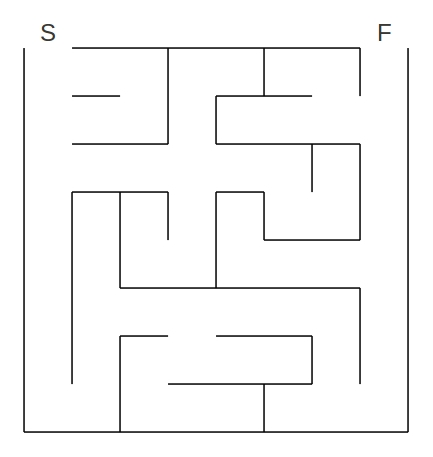
\includegraphics[width=3in]{./maze.jpg}
\end{center}
\begin{flushleft}
   Show how to model the maze as a graph.
\end{flushleft}

\vspace*{3.5in}

\begin{flushleft}
   Perform a breadth-first search on the maze to show how this algorithm can be used to find the shortest path from start to finish.
\end{flushleft}
\end{document} 
